% \renewcommand{\ldate}{2016-01-}
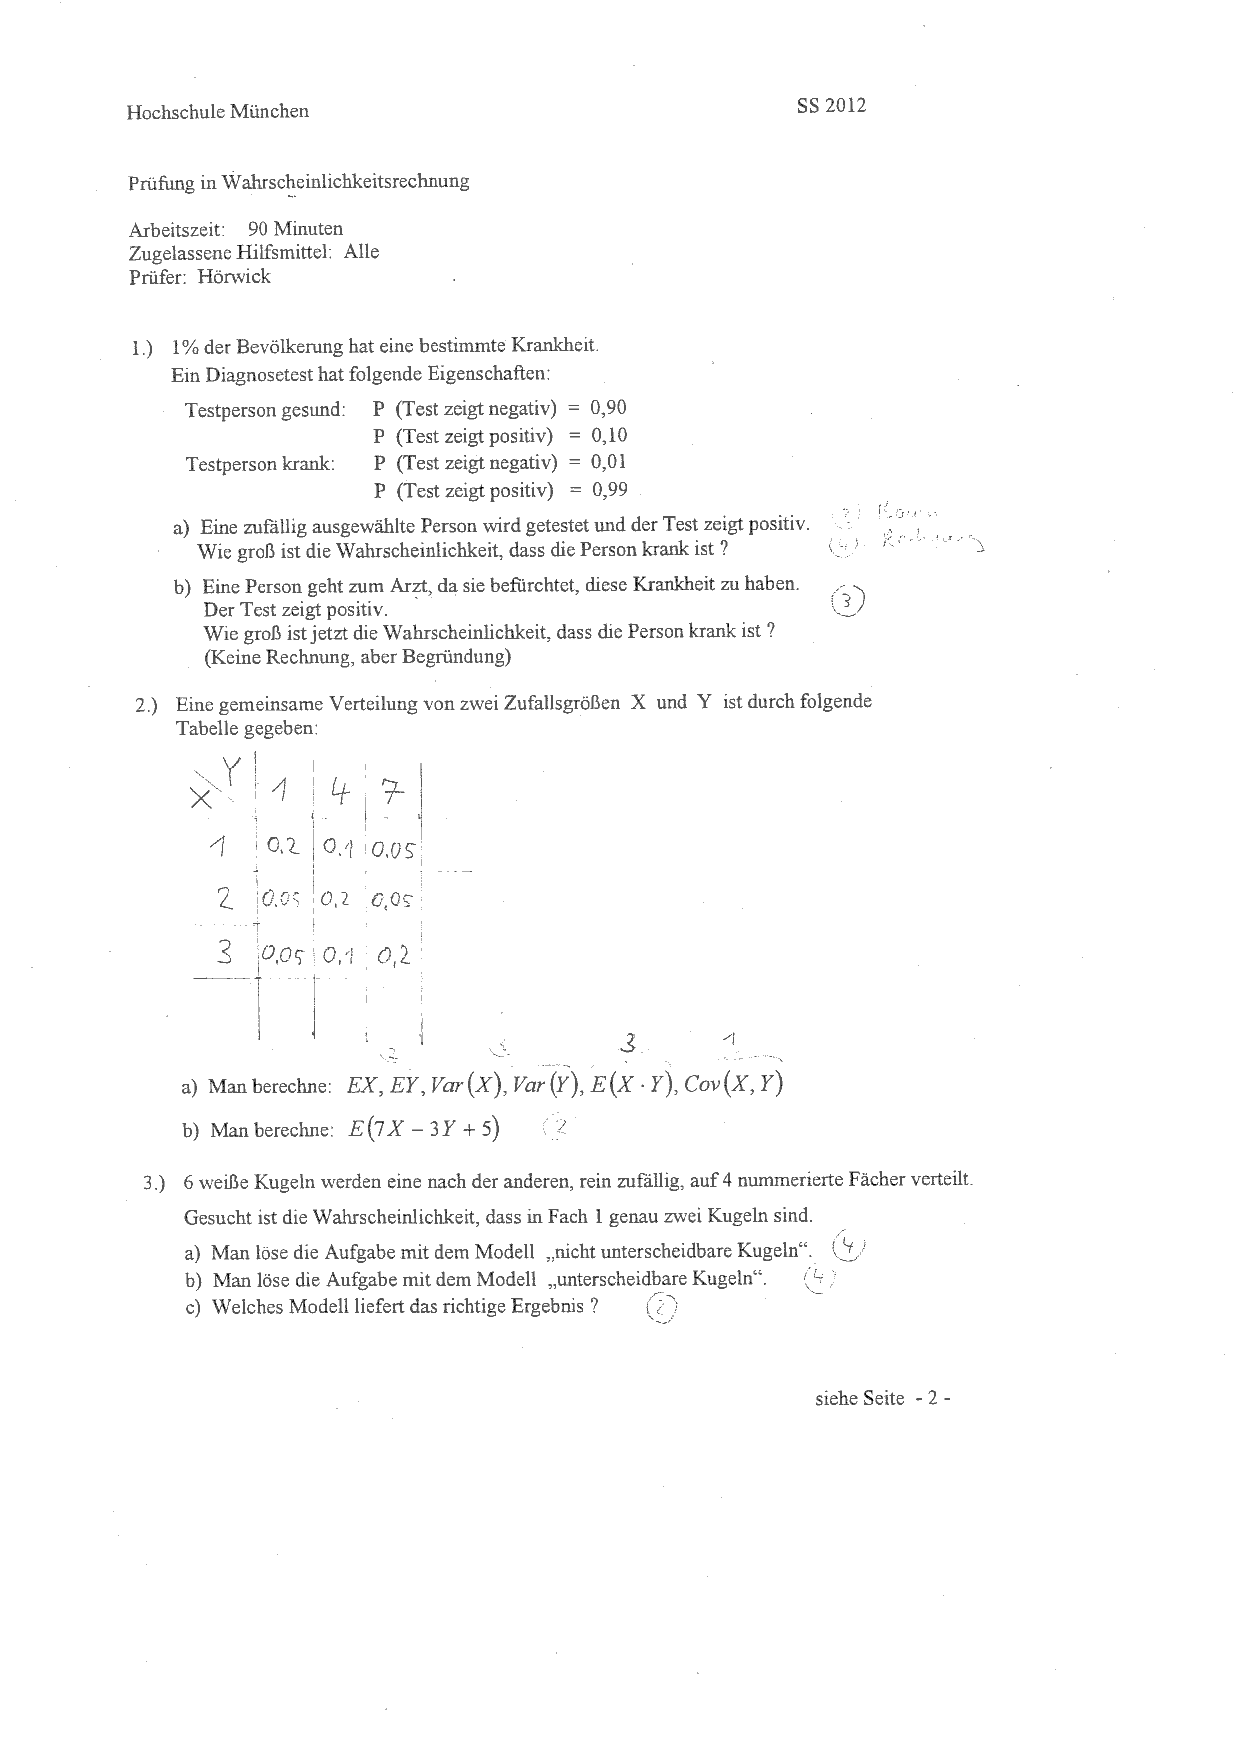
\includepdf[pages=-]{pruefungsangabe_wahrStat_ss2012}

\section{Lösung für die Prüfung SS 2012}

\subsection{zu 1)}
%1 \includegraphicsdeluxe{baumZuSs20121.jpg}{Wahrscheinlichkeitsbaum}{Wahrscheinlichkeitsbaum}{fig:baumZuSs20121}

\subsubsection{zu 1a)}
A: Person krank\\
B: Test zeigt positiv
$P(A|B) = \frac{P\cap B}{P(B)} = \frac{0.01\cdot 0.99}{0.01\cdot 0.99 + 0.99\cdot 0.10} = 0.09$

\subsubsection{zu 1b)}
Jetzt ist die apriori Wahrscheinlichkeit, dass er krank ist, höher (vielleicht 0.1 statt 0.01). Damit ist die aposteriori Wahrscheinlichkeit, dass er krank ist, auch höher (vielleicht 0.5). 

\subsection{zu 2a)}

\begin{tabular}{|c|c|c|c|c|}
\hline X/Y & 1 & 4 & 7 &  \\ 
\hline 1 & 0.2 & 0.1 & 0.05 & 0.35 \\ 
\hline 2 & 0.05 & 0.2 & 0.05 & 0.3 \\ 
\hline 3 & 0.05 & 0.1 & 0.2 & 0.35 \\ 
\hline  & 0.3 & 0.4 & 0.3 &  \\ 
\hline 
\end{tabular} 

\begin{enumerate}
\item Immer multiplizieren Zeile mal Randwahrscheinlichkeit: $ EX = 1\cdot 0.35 + 2\cdot 0.3 + 3\cdot 0.35 = 2$
\item Wert mal Wahrscheinlichkeit: $ 1\cdot 0.3 + 4\cdot 0.4 + 7\cdot 0.3 = 4$
\item $EX^2 = 1^2 \cdot 0.35 + 2^2\cdot 0.3 + 3^2\cdot 0.35 = 1\cdot 0.35 + 4\cdot 0.3 + 9\cdot 0.35 = 4.7$\\
$EY^2 = 1\cdot 0.3 + 16\cdot 0.4 + 49\cdot 0.3 = 21.4 $\\
$Var(X) = E(X^2) - (EX)^2 = 4.7 - 4 = 0.7$\\
$Var(Y) = E(Y^2) - (EY)^2 = 21.4 - 16 = 5.4$\\
\item Nicht einfach multiplizieren. Ganze Tabelle durchmachen: $ E(X\cdot Y) = 
1\cdot 1\cdot 0.2 + 
1\cdot 4\cdot 0.1 + 
1\cdot 7\cdot 0.05 + 
2\cdot 1\cdot 0.05 + 
2\cdot 4\cdot 0.2 + 
2\cdot 7\cdot 0.05 + 
3\cdot 1\cdot 0.05 + 
3\cdot 4\cdot 0.1 + 
3\cdot 7\cdot 0.2 = 8.9
$
\item $ Cov(X,Y) = E(X\cdot Y) - EX\cdot EX = 8.9 - 2 \cdot 4 = 0.9$
\end{enumerate}

\subsection{zu 2b)}
$ E(7X - 3Y + 5) = 7 EX - 3 EY + 5 = 7\cdot 2 - 3\cdot 4 + 5 = 7$

\subsection{zu 3)}
% 2 \includegraphicsdeluxe{UrnenmodellSS20123.jpg}{Urnenmodell}{Urnenmodell}{fig:UrnenmodellSS20123}

\subsubsection{zu 3a)}
Anzahl der Möglichkeiten bei n Fächern und k Kugeln: 
$ \binom{n+k-1}{k}, n=4, k=6 $

alle Möglichkeiten: $ \binom{4+6-1}{6} = \binom 9 6 = \binom 9 3 = \frac{9\cdot 8\cdot 7}{1\cdot 2\cdot 3} = 84$

günstige Möglichkeiten, also 4 Kugeln auf 3 Fächer: $ \binom{3+4-1}{4} = \binom 6 4 = \binom 6 2 = \frac{6\cdot 5}{1\cdot 2} = 15$

$\Rightarrow P = \frac{15}{84} = 0.178 $

\subsubsection{zu 3b)}
Formel bei n Fächern und k Kugeln für die Anzahl der Möglichkeiten: $ n^k $

alle Fälle: $4^6 = 4096 $

günstige Fälle: $ \binom 6 2 \cdot 3^4 = \frac{6\cdot 5}{1\cdot 2} \cdot 3^4 = 1215 $   

$\Rightarrow P = \frac{1215}{4096} = 0.296$

\subsubsection{zu 3c)}
b ist richtig, weil a falsch ist. a ist falsch, weil nicht alle Möglichkeiten gleich wahrscheinlich sind. 
% \profnote{Student: Warum sind nicht alle Möglichkeiten gleich wahrscheinlich. Professor: Mei, das ist halt so.}

\subsection{zu 4)}
\profnote{Durchschnitt heißt immer Erwartungswert}
$ X_1 $ Anzahl der Nieten bis zum 1. Treffer. 

$ X_2 $ Anzahl der Nieten vom 1. bis zum 2. Treffer. 

$ \vdots $

$ X_{12} $ Anzahl der Nieten vom 11. bis zum 12. Treffer. 

$ Y = X_1 + X_2 + ... + X_{12}$

$EY = E \sum_{i=1}^{12} X_i = EX_1 + ... + EX_{12} = 12\cdot EX_1 = 12 \cdot \frac{1-P}{P} = 12\cdot \frac{1-0.2}{0.2} = 48$ 
Im Schnitt sind es also 48 Nieten bis zum 12. Treffer. Dadurch braucht man im Schnitt 60 Versuche bis zum 12. Treffer. 

\subsection{zu 5)}
X: Anzahl der Tests pro Gruppe (10).

$ P(X=1) = 0.95^{10} = 0.6 $

$ P(X=11) = 0.40 $

$ EX = 1\cdot 0.60 + 11\cdot 0.40 = 5.0$

Pro Gruppe im Schnitt 5.0 Tests. Pro Person werden also im Schnitt 0.5 Tests benötigt. \\

\subsection{zu 6)}
% 3 \includegraphicsdeluxe{UrneSS2012z6.jpg}{Urne}{Urne}{fig:UrneSS2012z6}

\subsubsection{zu 6a)}
Mit Rücklegen 5 mal ziehen: $ P(\textrm{5 mal weiß}) = \rbr{\frac{7}{8}}^5 = 0.513 $

$ P(\textrm{mindestens einmal schwarz}) = 1 - 0.513 = 0.487 $